% =====================================================================
%  First-Divergence Consequence Analysis (FDCA)
%  Version 1.0.0 -- initial public archival release, August 2026
%  Munsik Kim, Independent Researcher, Seoul, Republic of Korea
%  Venue-neutral technical preprint. Not peer reviewed.
%
%  Build:
%    pdflatex FDCA_v1.0.0 ; bibtex FDCA_v1.0.0 ; pdflatex FDCA_v1.0.0 ; pdflatex FDCA_v1.0.0
%  (or: latexmk -pdf FDCA_v1.0.0.tex)
% =====================================================================

\documentclass[11pt,a4paper]{article}

% hyperref options must be registered before algorithm2e pulls it in
\PassOptionsToPackage{colorlinks=true,linkcolor=black,citecolor=black,urlcolor=blue}{hyperref}

\usepackage[T1]{fontenc}
\usepackage[utf8]{inputenc}
\usepackage{amsmath,amsthm}
\usepackage{newtxtext,newtxmath}  % embedded Times-like text and math fonts
\usepackage[scaled=0.9]{helvet}
\usepackage[margin=1in]{geometry}
\usepackage{booktabs}
\usepackage{array}
\usepackage{caption}
\usepackage{subcaption}
\usepackage{enumitem}
\usepackage{xcolor}
\usepackage{microtype}
\usepackage{tikz}
\usepackage{pgfplots}
\usepackage[ruled,vlined]{algorithm2e}
\usepackage{natbib}
\usepackage{fancyhdr}
\usepackage{hyperref}
\hypersetup{
  pdftitle={First-Divergence Consequence Analysis: From Quantization Onset to Perceptual Impact in Masked Visual Generators},
  pdfauthor={Munsik Kim},
  pdfsubject={Approximation error analysis for masked visual generative models},
  pdfkeywords={masked generative models, MaskGIT, post-training quantization,
    coupling, first divergence, total variation, LPIPS, DINOv2, reproducibility},
  pdfcreator={pdfLaTeX; FDCA v1.0.0 initial public release}
}

\usetikzlibrary{arrows.meta,positioning}
\pgfplotsset{compat=1.18}
\bibliographystyle{plainnat}

\theoremstyle{plain}
\newtheorem{theorem}{Theorem}[section]
\newtheorem{proposition}[theorem]{Proposition}
\theoremstyle{definition}
\newtheorem{definition}[theorem]{Definition}
\theoremstyle{remark}
\newtheorem{remark}[theorem]{Remark}

\newcommand{\TV}{\mathrm{TV}}
\newcommand{\Ind}[1]{\mathbf{1}\{#1\}}
\newcommand{\Ex}{\mathbb{E}}
\newcommand{\Prob}{\mathbb{P}}
\newcommand{\Mask}{\texttt{M}}
\newcommand{\diam}{\mathrm{diam}}
\newcommand{\rholabel}{\widetilde{\rho}}
\newcommand{\rhoatt}{\rho_{\mathrm{att}}}

\pagestyle{fancy}
\fancyhf{}
\fancyhead[L]{\small First-Divergence Consequence Analysis}
\fancyhead[R]{\small v1.0.0 (initial public release)}
\fancyfoot[C]{\thepage}
\renewcommand{\headrulewidth}{0.4pt}

\title{\bfseries First-Divergence Consequence Analysis:\\
From Quantization Onset to Perceptual Impact\\
in Masked Visual Generators}

\author{Munsik Kim\\
\small Independent Researcher, Seoul, Republic of Korea\\
\small ORCID: \href{https://orcid.org/0009-0008-9350-2435}{0009-0008-9350-2435}}

\date{Version 1.0.0 --- August 2026\\[2pt]
\small Technical preprint. Not peer reviewed. Venue-neutral layout.}

\begin{document}
\maketitle
\thispagestyle{fancy}

\begin{abstract}
\noindent
Approximation error in an iterative generator is usually measured in one of two
places. Local diagnostics report weight, activation, or logit distortion.
Endpoint diagnostics report image quality. Neither answers the question that sits
between them: at which step does the approximated sampler first behave
differently, and how much does that first difference eventually cost?

We study this question for a fixed monotone masked-decoding schedule whose
accepted token values are never revisited. \emph{First-Divergence Consequence
Analysis} (FDCA) runs a reference decoder and an approximate decoder from the
same anchor state under an explicit coupling, defines the \emph{first divergence}
as the first transition at which their states differ, and keeps apart two
quantities that endpoint scores collapse into one: how often a first split
occurs, and how much terminal damage follows given that it occurred. We prove a
pathwise stable-set bound, an exact onset--consequence decomposition, and a
coordinate-level innovation--influence envelope under explicit product-law and
hybrid-state assumptions.

We instantiate FDCA on official H-MaskGIT checkpoints with a branch-independent
Halton schedule, symmetric W8 post-training weight quantization,
conditional-form maximal coupling, and event-addressed random-number generation.
On H-MaskGIT-T, exact split incidence \emph{falls} from $0.213$ at target anchor label
$\rholabel=0.3$ to $0.130$ at $\rholabel=0.5$, while split-conditional LPIPS
\emph{rises} by $2.98\times$ and exact incidence-weighted LPIPS rises by
$1.77\times$. DINOv2 distance and a matched same-shock timing control move the
same way. Adding token-descendant features to a seed-only regression cuts
held-out LPIPS prediction error by $48.3\%$. On H-MaskGIT-S the conditional and
incidence-weighted ratios are $2.96\times$ and $1.92\times$, and every
preregistered replication test passes.

Onset and consequence therefore move in opposite directions across reverse
time, making split frequency insufficient as a standalone risk measure. All
claims are scoped to the audited Halton schedule, the specified coupling, a
one-step natural seed followed by a common approximate suffix, and operational
perceptual metrics.
\end{abstract}

\vspace{0.4em}
\noindent\fbox{\parbox{0.97\textwidth}{\small
\textbf{Scope of this release.}
The empirical program is frozen. Independent artifact audits cover the primary
perceptual study (H-MaskGIT-T) and the second-checkpoint replication
(H-MaskGIT-S), including zero controls, semantic RNG audits, complete token and
grid logging, MASK/clamp closure, and model-free reaggregation. The paper does
\emph{not} claim human perceptual ground truth, generality across architecture
families, coupling-independent behavior, or any guarantee about persistent
FP32-versus-W8 deployment.
}}

% =====================================================================
\section{Introduction}

Post-training approximation is now a standard part of deploying a generative
model. Quantization, caching, and approximate kernels all cut cost, and their
error is normally checked at one of two ends of the pipeline. At the near end we
measure how far the perturbed weights or logits sit from the originals. At the
far end we measure FID, a perceptual distance, or task accuracy. Neither
measurement says when the approximated generator first behaved differently, how
often that happens, or why two perturbations of the same local size can end up
costing very different amounts.

The gap matters most in iterative masked generators. A decoder predicts tokens,
commits a subset of positions, and moves on. Once one committed token differs
between an exact run and an approximate run, every later conditional is evaluated
on a different state, so the two runs are no longer comparable step by step.
Terminal error then depends on at least three separate objects: the probability
that a first split occurs at all, the geometry and severity of the token mismatch
it creates, and how sensitive the remaining decoding suffix is to that mismatch.
A single endpoint number hides all three. Reporting only the first --- how often
the runs diverge --- can reverse the risk ranking, which is what we find here.

We approach the problem with a paired stochastic analysis. A reference decoder
and an approximate decoder start from the same state and are joined by an
explicit coupling. The \emph{first divergence} is the first transition at which
their states differ. The stopping time itself is classical: first-disagreement
and maximal-agreement constructions have a long history
\citep{lindvall2002coupling,vollering2016maximal,ernst2019mexit}. What we add is
a consequence-aware specialization to monotone masked decoding, plus an
implementation contract that makes the resulting joint law auditable rather than
merely asserted.

The theory has two levels. A stable-set argument shows that coordinates already
fixed identically before the first split cannot contribute to terminal Hamming
damage; this gives a pathwise bound that holds for any coordinate-additive cost.
A time-ordered innovation--influence recursion then separates fresh same-state
implementation discrepancy from the propagation of mismatches that already exist.
The second level is useful as structure, but our experiments also mark its limit:
finite-panel neural influence profiles order the reverse-time regimes correctly
and then stop being informative inside a regime.

The empirical finding is simpler than the theory and does not depend on it. For
realistic W8 weight quantization, split incidence and conditional consequence
have opposite profiles across reverse time. Late transitions commit many
positions at once and therefore split often, but almost no decoding remains, so
the damage is small. Earlier transitions split rarely, yet the mismatch they
create is amplified through a long suffix and produces much larger token and
perceptual damage. The pattern survives natural quantization seeds, a matched
same-shock timing control, two perceptual metrics, and a second official
checkpoint.

\paragraph{Contributions.}
\begin{enumerate}[leftmargin=1.6em,itemsep=2pt]
\item \textbf{Theory.} We formulate FDCA for fixed monotone masked decoders and
prove three results: a stable-set first-divergence bound
(Theorem~\ref{thm:stableset}), an exact incidence--consequence decomposition
(Proposition~\ref{prop:decomp}), and a coordinate-level clipped
innovation--influence envelope (Theorem~\ref{thm:dag}).
\item \textbf{Measurement contract.} We specify, and then audit, what a paired
generative experiment has to fix in order to be reproducible: conditional-form
maximal coupling, event-addressed RNG, complete token-pair and pre/post-clamp
logging, semantic-key registries, zero controls, and model-free reaggregation
(Section~\ref{sec:contract}).
\item \textbf{Onset law under realistic quantization.} We connect W8 quantization
to the mismatch seeds it actually produces and to their closed-loop propagation.
Exact split incidence \emph{decreases} toward earlier reverse-time states while
conditional descendant damage \emph{increases} sharply
(Sections~\ref{sec:onset}--\ref{sec:propagate}).
\item \textbf{Perceptual bridge.} Conditional LPIPS, exact incidence-weighted
LPIPS, DINOv2 distance, and a matched timing control all show larger damage at
$\rholabel=0.5$ than at $\rholabel=0.3$, and the primary effects replicate on a second
official checkpoint (Sections~\ref{sec:perceptual}--\ref{sec:replication}).
\end{enumerate}

\paragraph{How to read the paper.}
Section~\ref{sec:setup} fixes notation and defines the three damage quantities
that carry most of the argument; readers who want only the empirical result can
go from there to Section~\ref{sec:results}. Section~\ref{sec:theory} is
self-contained and does not depend on the experiments.
Section~\ref{sec:negative} lists the results that failed and the boundaries they
impose.

% =====================================================================
\section{Related Work}

\subsection{Masked visual generation and schedule design}
MaskGIT introduced iterative bidirectional visual-token generation with
confidence-guided refinement \citep{chang2022maskgit}. Later work treats the
unmasking order as an algorithmic object in its own right. The Halton scheduler
replaces model-dependent confidence order with a spatially dispersed
low-discrepancy sequence \citep{halton1960efficiency,besnier2025halton}. Jump
Your Steps, factorized-approximation error bounds, and optimal inference
schedules characterize the cost of parallel unmasking
\citep{park2025jump,lavenant2025error,chen2026optimal}, and adaptive planning and
entropy-based methods push the same point further
\citep{kim2025train,peng2025path,benhamu2025accelerated,cai2026confidence}. These papers analyze sampler or scheduling bias. A complementary analysis of
the MaskGIT sampler makes its implicit temperature mechanism explicit and
introduces choose-then-sample and partial-caching variants
\citep{hayakawa2025demystifying}. We hold the pretrained decoder and a
branch-independent schedule fixed and study implementation approximation along
paired trajectories instead.

\subsection{Coupling and first disagreement}
Maximal-agreement coupling and MEXIT ask how long two stochastic processes can be
kept equal \citep{vollering2016maximal,ernst2019mexit}; the general machinery is
standard \citep{lindvall2002coupling,levin2017markov}. We use first divergence as
an onset variable and claim no novelty for the stopping time. Our addition is the
accounting that comes after the split, together with a contract that preserves
both branch marginals and keeps the reference draw invariant across coupling
families.

\subsection{Local influence}
Dobrushin-style comparison bounds control global discrepancy from local
conditional perturbations \citep{rebeschini2014comparison}. Our influence matrix
has the same single-site total-variation ancestry, but a fixed commit order makes
the dependency graph triangular and the horizon finite. The global suprema the
theorem needs are not computable for a neural decoder, so we keep the theorem and
the measured reachable-state profiles strictly separate and report the latter as
diagnostics.

\subsection{Approximate visual inference}
Caching and quantization are studied across masked, autoregressive, and
diffusion-style visual generators
\citep{yan2025lazymar,wu2025quantcache,moon2026shift}. Those methods optimize
throughput or endpoint quality. FDCA asks a different question: where does the
approximate implementation first change the stochastic trajectory, and what
happens to the state mismatch afterwards?

\subsection{Perceptual outcomes}
We use LPIPS as a learned paired perceptual distance
\citep{zhang2018unreasonable} and DINOv2 embeddings for an independent
representation-space check \citep{oquab2024dinov2}. A ResNet-50 classifier
\citep{he2016deep} supplies secondary distributional and label diagnostics. All
three are operational metrics and none is a substitute for human judgment.

% =====================================================================
\section{Setup and Notation}
\label{sec:setup}

\subsection{Fixed monotone masked decoder}
Let $I$ be a finite set of $N$ visual-token positions, $V$ a codebook, and
$\Mask \notin V$ a mask symbol. A \emph{branch-independent commit schedule} is an
ordered partition
\[
  \mathcal{C} = (C_1,\dots,C_K), \qquad \bigsqcup_{k=1}^{K} C_k = I ,
\]
whose blocks do not depend on either branch's realized tokens. Write
$D_k = \bigcup_{j\le k} C_j$ for the committed set and $U_k = I \setminus D_k$ for
the unresolved set. A state $x_k \in (V\cup\{\Mask\})^I$ is \emph{monotone} if a
position committed to a non-mask token is never revised.

For $u \in C_{k+1}$ the reference and approximate categorical laws are
$p_{k,u}(\cdot \mid x_k)$ and $q_{k,u}(\cdot \mid x_k)$. In the fixed-schedule
theoretical setting, the proposal laws over a commit batch factorize,
\[
  P_k(\cdot\mid x_k)=\bigotimes_{u\in C_{k+1}}p_{k,u}(\cdot\mid x_k),
  \qquad
  Q_k(\cdot\mid x_k)=\bigotimes_{u\in C_{k+1}}q_{k,u}(\cdot\mid x_k),
\]
and coordinate couplings use independently addressed random events conditional
on the common state. Both processes start from the same state and are joined by
a coupling $\Gamma$. We write $X_k$ for the reference state and $Y_k$ for the
approximate state. Factorization is needed for the product formula in
Equation~\eqref{eq:incidence}; the stable-set bound itself does not need it.

\begin{definition}[First divergence]
\label{def:tau}
The first-divergence time is $\tau = \inf\{k \ge 1 : X_k \neq Y_k\}$, with
$\tau = \dagger$ if the two branches never differ.
\end{definition}

Terminal discrepancy is measured with a weighted Hamming cost
\[
  d_\lambda(x,y) = \sum_{u \in I} \lambda_u \Ind{x_u \neq y_u},
  \qquad \lambda_u > 0, \quad \textstyle\sum_u \lambda_u = 1 ,
\]
and the paired terminal cost is $D^\Gamma = \Ex_\Gamma[d_\lambda(X_K,Y_K)]$.

\subsection{Reverse-time index and the unit of analysis}
\label{sec:rho}
The experiment selects five target anchor labels
$\rholabel\in\{0.1,0.3,0.5,0.7,0.9\}$ and then takes the nearest available
\emph{pre-transition} state in the audited 32-step Halton schedule. We write
$\rhoatt$ for the fraction actually unresolved in that state. Large values mean
\emph{early} in decoding and small values mean \emph{late}; ``reverse time''
always refers to this direction.

The distinction is material at the final anchor because the last Halton step
flushes all 41 remaining positions. Table~\ref{tab:anchors} gives the exact
schedule-derived values. Plots use the convenient target labels $\rholabel$ on
the horizontal axis; all laws and outcomes are computed at the corresponding
attained state $\rhoatt$.

\begin{table}[t]
\centering
\caption{Target labels and attained unresolved fractions on the frozen
$16\times16$, 32-step Halton schedule. Step numbers are one-indexed transition
numbers.}
\label{tab:anchors}
\small
\begin{tabular}{@{}ccccc@{}}
\toprule
Target $\rholabel$ & Transition & Unresolved before transition &
Attained $\rhoatt$ & Next commit batch \\
\midrule
0.1 & 32 & 41  & 0.16015625 & 41 \\
0.3 & 30 & 72  & 0.28125000 & 14 \\
0.5 & 24 & 126 & 0.49218750 & 8  \\
0.7 & 16 & 177 & 0.69140625 & 6  \\
0.9 & 6  & 231 & 0.90234375 & 5  \\
\bottomrule
\end{tabular}
\end{table}

The independent statistical unit is always the \emph{class--seed block}: one
ImageNet class label paired with one generation seed. Anchors, coupling
replicates, token positions, and image pairs inside a block are not independent
and are never treated as such.

\subsection{Three damage quantities, and why they differ}
\label{sec:threenumbers}
Most of the paper turns on keeping three numbers apart. Fix a target anchor regime
$\rholabel$ (with attained state $\rhoatt$) and let $S$ be the event that a first split occurs at the anchor
transition.

\begin{center}
\small
\begin{tabular}{@{}p{0.27\textwidth}p{0.31\textwidth}p{0.36\textwidth}@{}}
\toprule
\textbf{Quantity} & \textbf{Definition} & \textbf{Reads as} \\
\midrule
Exact split incidence &
$\Prob_\Gamma(S \mid \rholabel)$, exact under the specified coordinatewise coupling &
How often the approximation changes behavior here \\[4pt]
Split-conditional damage &
$\Ex_\Gamma[d \mid S,\rholabel]$ &
How bad it is when it does \\[4pt]
Incidence-weighted damage &
$\Prob_\Gamma(S\mid\rholabel)\,\Ex_\Gamma[d\mid S,\rholabel]$ &
Expected damage attributable to a split at this anchor \\
\bottomrule
\end{tabular}
\end{center}

\medskip
Incidence is not estimated by counting splits in a Monte Carlo run. Under the
coupling of Section~\ref{sec:coupling} it is available in closed form from the
per-position total variations, which removes one source of noise from every
downstream contrast.

\begin{table}[t]
\centering
\caption{Notation used throughout.}
\label{tab:notation}
\small
\begin{tabular}{@{}ll@{}}
\toprule
Symbol & Meaning \\
\midrule
$I$, $N$ & set of visual-token positions; $N=|I|$ \\
$\mathcal{C}=(C_1,\dots,C_K)$ & branch-independent commit schedule, $K$ steps \\
$U_k$, $\rholabel$, $\rhoatt$ & unresolved set; target label; attained unresolved fraction \\
$p_{k,u},\ q_{k,u}$ & reference (FP32) and approximate (W8) conditional laws at $u$ \\
$X_k,\ Y_k$ & reference and approximate states \\
$\tau$ & first-divergence time (Definition~\ref{def:tau}) \\
$d_\lambda$ & weighted terminal Hamming cost \\
$b_u=\TV(p_u,q_u)$ & per-position direct total variation ("direct TV") \\
$h_k(s)$, $m_k(s)$ & one-step split hazard; split-conditional terminal consequence \\
$s_u$, $M_{uv}$ & same-state innovation at $u$; single-site influence of $v$ on $u$ \\
$S_{\mathrm{seed}}$ & set of coordinates that differ at the first split \\
descendant & a coordinate that differs at the end but was not in $S_{\mathrm{seed}}$ \\
block & one class--seed pair; the independent unit of analysis \\
\bottomrule
\end{tabular}
\end{table}

% =====================================================================
\section{First-Divergence Consequence Analysis}
\label{sec:theory}

\subsection{Stable-set first-divergence bound}

\begin{definition}[Future-stable set]
At a common state $s$ immediately before transition $k+1$, a set $F_k(s)$ is
future-stable if every $u\in F_k(s)$ is equal in both branches and, under every
allowed continuation of either branch, coordinate $u$ is never revised. We
suppress $k$ when the stage is determined by the state.
\end{definition}

\begin{theorem}[Stable-set consequence bound]
\label{thm:stableset}
Let $d(x,y) = \sum_u \lambda_u c_u(x_u,y_u)$ be any coordinate-additive terminal
cost. Then, pathwise,
\[
  d(X_K,Y_K) \;\le\;
  \begin{cases}
    \displaystyle\sum_{u \notin F(X_{\tau-1})} \lambda_u \diam(c_u)
      & \text{on } \{\tau \neq \dagger\},\\[10pt]
    0 & \text{on } \{\tau = \dagger\},
  \end{cases}
\]
and consequently
$D^\Gamma \le \Ex_\Gamma\!\left[R(X_{\tau-1})\,\Ind{\tau \neq \dagger}\right]$,
where $R(s) = \sum_{u \notin F(s)} \lambda_u \diam(c_u)$ is the total cost mass
outside the future-stable set.
\end{theorem}

For uniform token Hamming cost under the audited Halton schedule, $R(s)$ is the
fraction of positions that can still be affected. The bound is exact in scope and
cheap to evaluate, but it is loose whenever the first split lands early and $R(s)$
is close to one. It states what \emph{can} be damaged, not what typically is.

\subsection{Incidence and consequence}

Let $G_k = \{\tau > k\}$. At a common state $s$, define the one-step split hazard
and the conditional terminal consequence
\[
  h_k(s) = \Prob\big(X_{k+1} \neq Y_{k+1} \,\big|\, G_k,\ X_k = Y_k = s\big),
  \qquad
  m_k(s) = \Ex\big[d_\lambda(X_K,Y_K) \,\big|\, G_k,\ X_k = Y_k = s,\ \tau = k+1\big].
\]
When $h_k(s)=0$, the conditional law defining $m_k(s)$ is immaterial; we adopt
the convention $h_k(s)m_k(s)=0$.

\begin{proposition}[Exact onset--consequence decomposition]
\label{prop:decomp}
\[
  D^\Gamma \;=\; \sum_{k=0}^{K-1}
  \Ex\!\left[\Ind{G_k}\, h_k(X_k)\, m_k(X_k)\right].
\]
For a single target anchor $\rholabel$ the empirical form is
$\Ex[D \mid \rholabel] = \Prob(\text{split} \mid \rholabel)\,\Ex[D \mid \text{split},\rholabel]$.
\end{proposition}

The identity is elementary. Its value is entirely in what it licenses: the split
law, the seed geometry, and the downstream consequence can be estimated by three
separate procedures, each with its own controls, and only then multiplied.

\subsection{Innovation--influence accounting}

For each commit stage let $\mathcal{S}_k$ be an admissible state class closed
under the single-coordinate hybrid substitutions used below. The same-state
implementation discrepancy at a future position $u$ is
\[
  s_u = \sup_{x \in \mathcal{S}_k}
  \TV\big(p_{k,u}(\cdot \mid x),\,q_{k,u}(\cdot \mid x)\big),
\]
and for $v$ committed before $u$ the single-site influence is
\[
  M_{uv} = \sup_{\substack{x,y \in \mathcal{S}_k\\x\sim_v y}}
  \TV\big(q_{k,u}(\cdot \mid x),\,q_{k,u}(\cdot \mid y)\big),
\]
where $x\sim_v y$ means that $x$ and $y$ differ only at coordinate $v$. Hybrid
closure is a theorem assumption; a measured collection of reachable states is
not a substitute for it.

\begin{theorem}[Clipped DAG envelope]
\label{thm:dag}
Order positions by commit time and define
\[
  \bar r_u = \min\Big(1,\; s_u + \sum_{v \prec u} M_{uv}\, \bar r_v\Big).
\]
Under coordinatewise maximal coupling,
$\Prob(X_K[u] \neq Y_K[u]) \le \bar r_u$ and $D^\Gamma \le \lambda^\top \bar r$.
\end{theorem}

Because influence flows only from strictly earlier commit blocks, $M$ is strictly
block-triangular with $K$ blocks. Hence $M^K = 0$ and
\[
  (I - M)^{-1} \;=\; \sum_{j=0}^{K-1} M^{j}
\]
exists with no contraction assumption. Finiteness comes from nilpotency, not from
a spectral condition.

\begin{remark}[Measured profiles are not certificates]
\label{rem:notcert}
Theorem~\ref{thm:dag} is stated with suprema over all admissible states. For a
neural decoder those suprema are out of reach. What we can measure are
reachable-state local influences, calibration quantiles, or finite-panel maxima.
Such profiles are legitimate diagnostics and we report them as such, but they do
not inherit the theorem's global language. Section~\ref{sec:negative} gives the
practical cost of the gap: measured profiles order the reverse-time regimes
correctly and then add almost nothing inside a regime.
\end{remark}

\subsection{Single shock versus persistent approximation}
\label{sec:estimands}

Two estimands differ in where innovation comes from, and they must not be
conflated.

\emph{Single shock with common suffix.} One transition is allowed to differ,
creating a seed mismatch set $E$. After that, both branches run the same
approximate kernel. Future same-state innovation is zero, so the experiment
isolates state-mediated propagation.

\emph{Persistent approximation.} The reference branch keeps using $p$ and the
approximate branch keeps using $q$ for the whole suffix. Fresh innovation
continues after the first split and has to be counted. A seed-only recursion is
invalid for this estimand; the finite-state audit in Appendix~\ref{app:program}
includes a counterexample where omitting future innovation strictly
underestimates the terminal cost.

The strongest experiments in this paper use a natural one-step seed followed by a
common approximate suffix. The seed comes from the real FP32-versus-W8 one-step
law, and propagation is then observed under a common W8 suffix. Everything we
report about propagation is scoped to that estimand.

% =====================================================================
\section{Measurement Contract}
\label{sec:contract}

A paired stochastic experiment is reproducible only if the joint law is pinned
down by the code rather than by the description. This section states the contract
that was frozen and audited before any headline number was computed.

\begin{figure}[t]
\centering
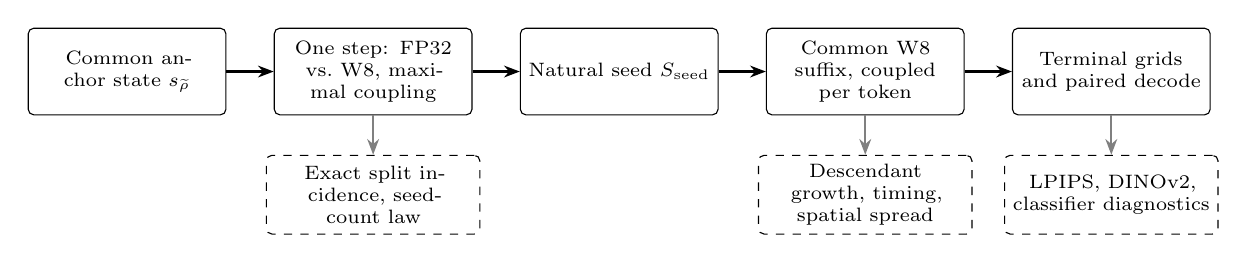
\begin{tikzpicture}[
  node distance=5mm and 6mm,
  box/.style={draw,rounded corners=2pt,align=center,inner sep=3pt,
              font=\scriptsize,minimum height=11mm,text width=23mm},
  diag/.style={draw,dashed,rounded corners=2pt,align=center,inner sep=3pt,
              font=\scriptsize,text width=25mm,minimum height=10mm},
  arr/.style={-{Stealth[length=2mm]},thick}
]
\node[box] (anchor) {Common anchor state $s_{\rholabel}$};
\node[box,right=of anchor] (step) {One step: FP32 vs.\ W8, maximal coupling};
\node[box,right=of step] (seed) {Natural seed $S_{\mathrm{seed}}$};
\node[box,right=of seed] (suffix) {Common W8 suffix, coupled per token};
\node[box,right=of suffix] (term) {Terminal grids and paired decode};

\draw[arr] (anchor) -- (step);
\draw[arr] (step) -- (seed);
\draw[arr] (seed) -- (suffix);
\draw[arr] (suffix) -- (term);

\node[diag,below=of step] (o1) {Exact split incidence, seed-count law};
\node[diag,below=of suffix] (o2) {Descendant growth, timing, spatial spread};
\node[diag,below=of term] (o3) {LPIPS, DINOv2, classifier diagnostics};

\draw[arr,gray] (step) -- (o1);
\draw[arr,gray] (suffix) -- (o2);
\draw[arr,gray] (term) -- (o3);
\end{tikzpicture}
\caption{The natural-shock experiment. The reference and approximate kernels
differ for exactly one transition. After the natural seed is created, both
branches use the same W8 suffix, which isolates propagation from any further
implementation innovation.}
\label{fig:pipeline}
\end{figure}

\subsection{Generator and schedule}
We use the official PyTorch Halton-MaskGIT implementation at source revision \texttt{f61b0a1} (full commit:\allowbreak
\nolinkurl{f61b0a1314717004dc7487531fd16a8bb71e1888})
\citep{besnier2025halton}. The primary checkpoint is
\texttt{ImageNet\_256\_tiny.pth} (H-MaskGIT-T; hidden width 384, depth 6,
6 attention heads) and the replication checkpoint is
\texttt{ImageNet\_256\_small.pth} (H-MaskGIT-S; hidden width 512, depth 12,
6 heads; 69,344,769 loaded parameters). The Small checkpoint is pinned to Hugging
Face revision \texttt{ffc7fd4} (full revision:\allowbreak
\nolinkurl{ffc7fd4c5fc7b16010acc4aa342310484d7de62a}); its
external-byte ledger records size 832,274,338 and SHA-256
\texttt{760b9937...07fb0e2}. Both configurations use a $16\times16$ token grid
and 32 sampling steps. The Halton schedule with
\texttt{randomize=False} supplies a branch-independent sequence of disjoint
commit sets, and source inspection plus trajectory audits confirm that
previously committed token values are never revised.

We also audited the confidence sampler and then excluded it from the exact
theorem. Its \emph{occupancy} is monotone, but committed token \emph{values} can
be rewritten. That distinction decides which sampler Theorem~\ref{thm:stableset}
applies to, and it is easy to miss.

\subsection{Approximation contract}
The reference model uses FP32 weights. The approximate model applies
deterministic symmetric per-output-channel round-to-nearest quantization to
eligible transformer linear weights:
\[
  Q_b(W_{o,:}) = \mathrm{clip}\!\left(
    \mathrm{round}(W_{o,:}/\Delta_o),\, -q_{\max},\, q_{\max}\right)\Delta_o,
  \qquad
  \Delta_o = \frac{\max_j |W_{o,j}|}{q_{\max}} .
\]
For an all-zero output row we set $Q_b(W_{o,:})=0$ directly. The implementation
uses deterministic PyTorch \texttt{round} (ties to even) and zero point 0. The
primary realistic cell is W8 with $q_{\max}=127$. Activations, norms,
embeddings, biases, and the VQ decoder stay in FP32. W4 is retained only as a
saturated stress regime (Section~\ref{sec:w4}).

\subsection{Conditional-form maximal coupling}
\label{sec:coupling}
For categorical laws $p$ and $q$, the reference token is drawn first and
preserved across comparison families; the approximate token is then either
accepted or drawn from the positive residual (Algorithm~\ref{alg:coupling}).
Drawing the reference token first is not cosmetic. It keeps the reference
trajectory identical across coupling variants, so a paired contrast cannot be
contaminated by a change of reference draw.

\begin{algorithm}[t]
\caption{Conditional-form maximal coupling for one token}
\label{alg:coupling}
\KwIn{categorical laws $p,q$; semantic keys $k_x,k_a,k_r$}
$x \leftarrow \textsc{InverseCDF}(p,\,U(k_x))$\;
\If{$\TV(p,q)=0$}{\Return $(x,x)$\;}
$a \leftarrow \min\{1,q(x)/p(x)\}$\tcp*{$p(x)>0$ almost surely under $x\sim p$}
\eIf{$U(k_a)\le a$}{
  \Return $(x,x)$\;
}{
  $r \leftarrow (q-p)_+/\TV(p,q)$\;
  $y \leftarrow \textsc{InverseCDF}(r,\,U(k_r))$\;
  \Return $(x,y)$\;
}
\end{algorithm}

The construction satisfies $X \sim p$, $Y \sim q$, and
$\Prob(X \neq Y) = \TV(p,q)$. When the commit-batch laws factorize as in Section~\ref{sec:setup} and the
coordinate couplings use independent semantic events, applying the construction
over a fixed batch $C$ gives the exact split incidence under this specified
coordinatewise coupling:
\begin{equation}
\label{eq:incidence}
  h_{\mathrm{split}} = 1 - \prod_{u \in C} (1 - b_u),
  \qquad b_u = \TV(p_u,q_u) .
\end{equation}
This coupling is optimal for each coordinate's mismatch probability. It is not
optimal for the whole path or for any terminal image metric, and we make no such
claim.

\subsection{Event-addressed random-number generation}
Sequential PRNG consumption silently changes the coupling whenever branch order,
batching, or a rejection loop changes. Every random event is therefore addressed
by a semantic key:
\begin{center}\ttfamily\small
EventKey(experiment\_id, model\_cell, block\_id, anchor\_id,\\
replicate\_id, attempt\_id, step, position, event\_kind, draw\_id)
\end{center}
Distinct event kinds separate reference proposals, accept/reject draws, and
residual draws. Runtime registries and model-free reconstruction classify
intentional reference-stream reuse and fail on any unclassified duplicate. Across
the final primary studies, unclassified duplicates and missing expected keys are
both zero.

\subsection{State and artifact logging}
The logging contract retains far more than terminal metrics: every selected token
pair including equal pairs; seed and descendant coordinate vectors at each step;
terminal pre-clamp and post-clamp token grids; selected-MASK and clamp-induced
changes; decoded tensor, image, feature, and preprocessing hashes; source,
checkpoint, and metric weight hashes; and class--seed block manifests, semantic
RNG manifests, and source-to-claim tables.

A dedicated replay stage (P2B) covers more than two million selected token pairs
and finds no equal-MASK and no one-sided-MASK event under the frozen P2N law. The
final perceptual studies record zero selected-MASK events and zero clamp-induced
changes.

% =====================================================================
\section{Experimental Design}
\label{sec:design}

\subsection{Anchors and blocks}
The primary perceptual study uses target labels $\rholabel \in \{0.1, 0.3, 0.5, 0.7, 0.9\}$ on 48
new class--seed blocks. The confirmatory replication uses the preregistered
primary contrast $\rholabel = 0.5$ versus $\rholabel = 0.3$ on 40 power-selected new
blocks. Every stage excludes all blocks used by its predecessors, so no block is
reused across scientific stages.

\subsection{Natural seed and common suffix}
At an anchor state we compute the FP32 and W8 laws on the same next commit batch.
The one-step natural seed is sampled with Algorithm~\ref{alg:coupling}, and
conditional on a split the exact seed vector is retained, including multi-seed
cases. Both branches then run the same W8 decoder over the same fixed Halton
suffix. This removes further FP32-versus-W8 innovation and isolates the
downstream effect of the seed, as sketched in Figure~\ref{fig:pipeline}.

Two controls sit alongside the main panel. A matched timing panel inserts the
same source-coordinate and token substitution at $\rholabel=0.3$ and $\rholabel=0.5$ within
a block, which removes shock-identity variation between the two regimes.
Zero-seed controls set both post-transition states equal and then verify exact
token, image, and metric equality end to end.

\subsection{Perceptual and semantic metrics}
The primary metric is LPIPS with the AlexNet backbone
\citep{zhang2018unreasonable}. DINOv2 ViT-S/14 cosine distance provides a
separate representation-space outcome \citep{oquab2024dinov2}. A pinned ResNet-50
supplies Jensen--Shannon divergence, top-1 disagreement, and conditioning-class
probability and logit diagnostics. SSIM and pixel $L_1$ are low-level secondary
measures. Metric weights, preprocessing, batch shape, and numerical tolerances
were frozen before any outcome was loaded. LPIPS exceeded the
scalar-versus-batch tolerance during smoke testing, so the preregistered scalar
fallback was used.

\subsection{Statistical tests}
All headline contrasts use 20{,}000 paired block-bootstrap resamples over
class--seed blocks. The primary perceptual hypotheses compare $\rholabel=0.5$ with
$\rholabel=0.3$ on conditional LPIPS, exact incidence-weighted LPIPS, conditional
DINOv2 distance, and matched same-shock LPIPS. A ratio threshold of $1.5$ and a
positive lower bootstrap endpoint were preregistered. The token-to-perceptual
link is tested by leave-one-block-out ridge regression, comparing a seed-only
model against a model that adds descendant count and rate, timing, and spatial
spread.

\subsection{Audit chain}
Table~\ref{tab:audit} summarizes the load-bearing controls. The P2P package
passes a 3{,}170-entry run manifest with zero mismatches and 60 of 60 frozen
tests. P3S passes 1{,}429 of 1{,}429 run-manifest entries, 52 pytest categories,
and 60 generated audit assertions. The P3S Full-package count is 1{,}431 because
it adds two archive-level bookkeeping files to the 1{,}429 run artifacts; these
are not extra scientific outputs. One gap is worth stating plainly: the
H-MaskGIT-S checkpoint bytes sit outside the review archive. The frozen filename,
revision, size, and SHA ledger are audited, but the archive audit does not rehash
the external 832\,MB file.

\begin{table}[t]
\centering
\caption{Technical audit summary for the final perceptual study and the
replication.}
\label{tab:audit}
\footnotesize
\begin{tabular}{@{}>{\raggedright\arraybackslash}p{0.27\textwidth} >{\raggedright\arraybackslash}p{0.325\textwidth} >{\raggedright\arraybackslash}p{0.325\textwidth}@{}}
\toprule
Audit item & H-MaskGIT-T (P2P) & H-MaskGIT-S (P3S) \\
\midrule
New scientific blocks & 48; predecessor overlap 0 & 40; predecessor overlap 0 \\
Zero controls & 288 exact token/image/metric matches & 112 exact token/image/metric matches \\
Selected-MASK / clamp changes & 0 / 0 & 0 / 0 \\
Unclassified / missing RNG keys & 0 / 0 & 0 / 0 \\
Complete seed-token pairs & 135{,}514 & 55{,}314 \\
Terminal token grids & $1{,}920+192+96+288=2{,}496$ & $640+160+80+128+32=1{,}040$ \\
Model-free reaggregation & PASS; max discrepancy 0 & PASS; secondary discrepancy 0 \\
Test inventory & 60/60 frozen tests & 52 pytest categories + 60 audit assertions \\
Package/run manifests & 3{,}170 entries; mismatch 0 & 1{,}431 Full, 151 Summary, 1{,}429 run; mismatch 0 \\
\bottomrule
\end{tabular}
\end{table}

% =====================================================================
\section{Results}
\label{sec:results}

\subsection{The onset law: many late splits, rare early splits}
\label{sec:onset}

For H-MaskGIT-T under W8, the mean per-position direct TV is close to constant
across reverse time at roughly $0.017$. Split incidence nonetheless varies by a
factor of six, and Equation~\eqref{eq:incidence} says why: the Halton schedule
commits a very different number of positions per step. At the latest target anchor $\rholabel=0.1$ (attained $\rhoatt=0.1602$), the
next batch holds 41 positions and exact incidence is $0.501$. At target $\rholabel=0.5$ (attained $\rhoatt=0.4922$), it
holds eight positions and incidence is $0.130$. The onset law measured on the P2P
blocks matches the independently generated P2N blocks closely.

\begin{table}[t]
\centering
\caption{H-MaskGIT-T under W8: exact onset law and split-conditional perceptual
consequence. Incidence falls and consequence rises as the target anchor label $\rholabel$ increases.}
\label{tab:onset}
\small
\begin{tabular}{@{}ccccccc@{}}
\toprule
$\rholabel$ & $\rhoatt$ & Next batch & Split incidence & $\Ex|S_{\mathrm{seed}}|$
& Conditional LPIPS & Conditional DINOv2 \\
\midrule
0.1 & 0.1602 & 41 & 0.5008 & 0.6939 & 0.00444 & 0.00344 \\
0.3 & 0.2813 & 14 & 0.2132 & 0.2382 & 0.01013 & 0.00743 \\
0.5 & 0.4922 &  8 & 0.1298 & 0.1379 & 0.03013 & 0.02227 \\
0.7 & 0.6914 &  6 & 0.1021 & 0.1067 & 0.07594 & 0.05634 \\
0.9 & 0.9023 &  5 & 0.0833 & 0.0863 & 0.21451 & 0.15240 \\
\bottomrule
\end{tabular}
\end{table}

\begin{figure}[t]
\centering
\begin{subfigure}{0.47\textwidth}
\centering
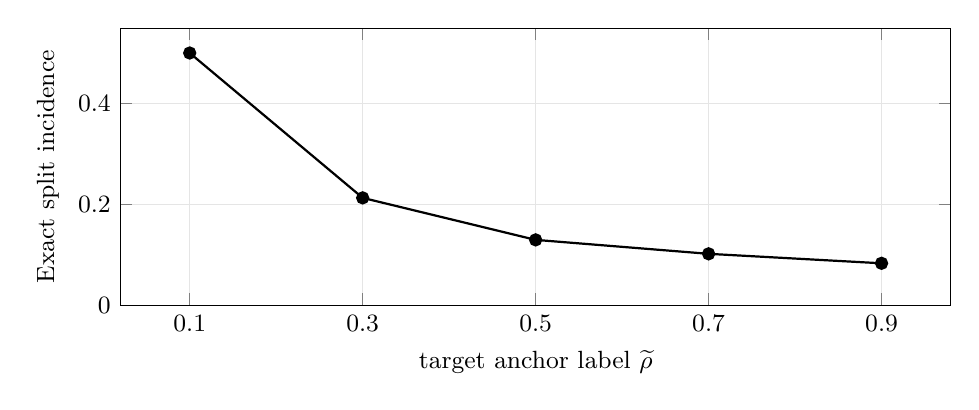
\begin{tikzpicture}
\begin{axis}[
  width=\textwidth, height=5.1cm,
  xlabel={target anchor label $\rholabel$}, ylabel={Exact split incidence},
  xtick={0.1,0.3,0.5,0.7,0.9}, ymin=0, ymax=0.55,
  grid=major, grid style={gray!20}, tick label style={font=\small},
  label style={font=\small}]
\addplot[thick,mark=*,color=black]
  coordinates {(0.1,0.5008)(0.3,0.2132)(0.5,0.1298)(0.7,0.1021)(0.9,0.0833)};
\end{axis}
\end{tikzpicture}
\caption{Onset incidence falls as decoding moves earlier.}
\end{subfigure}\hfill
\begin{subfigure}{0.47\textwidth}
\centering
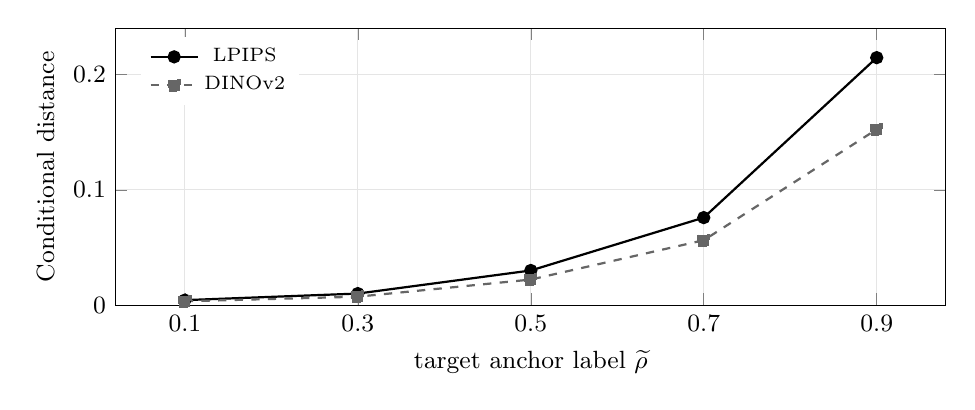
\begin{tikzpicture}
\begin{axis}[
  width=\textwidth, height=5.1cm,
  xlabel={target anchor label $\rholabel$}, ylabel={Conditional distance},
  xtick={0.1,0.3,0.5,0.7,0.9}, ymin=0, ymax=0.24,
  legend pos=north west, legend style={font=\scriptsize,draw=none},
  grid=major, grid style={gray!20}, tick label style={font=\small},
  label style={font=\small}]
\addplot[thick,mark=*,color=black]
  coordinates {(0.1,0.00444)(0.3,0.01013)(0.5,0.03013)(0.7,0.07594)(0.9,0.21451)};
\addlegendentry{LPIPS}
\addplot[thick,mark=square*,dashed,color=black!60]
  coordinates {(0.1,0.00344)(0.3,0.00743)(0.5,0.02227)(0.7,0.05634)(0.9,0.15240)};
\addlegendentry{DINOv2}
\end{axis}
\end{tikzpicture}
\caption{Conditional consequence rises sharply.}
\end{subfigure}
\caption{Opposing reverse-time profiles for H-MaskGIT-T under W8. The
horizontal axis uses target labels $\rholabel$; attained fractions are listed in
Table~\ref{tab:onset}. Splits are most frequent late in decoding, where little
suffix remains; conditional perceptual damage is largest early, where a great
deal remains.}
\label{fig:opposing}
\end{figure}

\subsection{Natural seeds propagate through the suffix}
\label{sec:propagate}

The natural W8 split is usually sparse. At $\rholabel=0.3$ and $\rholabel=0.5$, about
$89\%$ and $94\%$ of split events contain exactly one seed coordinate, which is
what the seed-count means in Table~\ref{tab:onset} imply. Conditional descendant
rates are $0.0375$ and $0.0848$, a ratio of $2.26$. These rates are normalized
by the number of remaining propagation-opportunity coordinates, so the contrast
is not a mechanical consequence of the earlier anchor having more unresolved
positions. At $\rholabel=0.5$, $97.4\%$ of
natural split replicates create at least one descendant mismatch, so extinction
of the seed is the exception rather than the rule. The matched same-shock timing
control yields a comparable twofold token-level contrast, which separates the
effect of reverse-time position from the identity of the shock.

\subsection{Perceptual consequence on H-MaskGIT-T}
\label{sec:perceptual}

Table~\ref{tab:primary} reports the preregistered P2P hypotheses. All four pass
the $1.5\times$ ratio threshold with positive lower bootstrap endpoints.

\begin{table}[t]
\centering
\caption{Primary H-MaskGIT-T perceptual results, target $\rholabel=0.5$ versus $\rholabel=0.3$.
Intervals are 95\% paired block-bootstrap intervals over 48 class--seed blocks.}
\label{tab:primary}
\small
\begin{tabular}{@{}lccccc@{}}
\toprule
Outcome & $\rholabel=0.5$ & $\rholabel=0.3$ & Ratio & Difference & 95\% CI for difference \\
\midrule
Conditional LPIPS        & 0.03013  & 0.01013  & 2.975 & 0.02000  & $[0.01719,\ 0.02287]$ \\
Incidence-weighted LPIPS & 0.003927 & 0.002213 & 1.775 & 0.001714 & $[0.001368,\ 0.002066]$ \\
Conditional DINOv2       & 0.02227  & 0.00743  & 2.996 & 0.01484  & $[0.01099,\ 0.01878]$ \\
Matched same-shock LPIPS & 0.04004  & 0.01495  & 2.678 & 0.02509  & $[0.01552,\ 0.03588]$ \\
\bottomrule
\end{tabular}
\end{table}

The conditional LPIPS contrast is positive in 47 of the 48 blocks. It stays
positive under block medians, under restriction to single-seed events, after
excluding extinctions, after removing the top $1\%$ of rows, and after adjusting
for seed severity. DINOv2 gives an almost identical reverse-time ratio despite
being a different metric on a different backbone. In the matched timing panel,
where the source coordinate and the alternative token are held fixed inside each
block, the $\rholabel=0.5$ damage is still $2.68\times$ larger.

\subsection{Incidence offsets consequence without cancelling it}
\label{sec:attribution}

Exact split incidence is lower at $\rholabel=0.5$ than at $\rholabel=0.3$, so the two
effects push against each other in the unconditional metric. Writing $\bar h$ and
$\bar m$ for the block-aggregated incidence and conditional damage, a symmetric
two-factor attribution of the unconditional LPIPS difference is
\[
  \Delta_{\text{incidence}} = (\bar h_{.5} - \bar h_{.3})\,
    \frac{\bar m_{.5} + \bar m_{.3}}{2},
  \qquad
  \Delta_{\text{consequence}} = (\bar m_{.5} - \bar m_{.3})\,
    \frac{\bar h_{.5} + \bar h_{.3}}{2},
\]
which evaluates to
\[
  \Delta_{\text{incidence}} = -0.001743, \qquad
  \Delta_{\text{consequence}} = +0.003457, \qquad
  \Delta_{\text{total}} = +0.001714 .
\]
The incidence term removes about half of the consequence term, and what is left
is still positive.\footnote{Both terms are computed from per-block aggregates in
the frozen analysis, not from the rounded anchor means printed in
Table~\ref{tab:onset}. Recomputing from those rounded means shifts the individual
terms in the third decimal place and leaves the signs and the total unchanged.}
The attribution is descriptive rather than unique: a sequential decomposition
assigns the interaction term differently, and we read no causal weight into
either factor.

\begin{figure}[t]
\centering
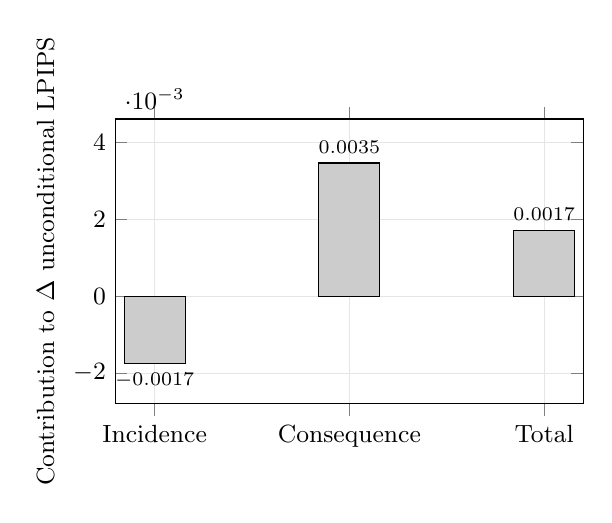
\begin{tikzpicture}
\begin{axis}[
  width=0.62\textwidth, height=5.2cm,
  ybar, bar width=22pt,
  symbolic x coords={Incidence, Consequence, Total},
  xtick=data, ymin=-0.0028, ymax=0.0046,
  ylabel={Contribution to $\Delta$ unconditional LPIPS},
  nodes near coords, nodes near coords style={font=\scriptsize},
  every node near coord/.append style={/pgf/number format/fixed,
      /pgf/number format/precision=4},
  grid=major, grid style={gray!20},
  tick label style={font=\small}, label style={font=\small}]
\addplot[fill=black!20,draw=black]
  coordinates {(Incidence,-0.001743) (Consequence,0.003457) (Total,0.001714)};
\end{axis}
\end{tikzpicture}
\caption{Opposing contributions to the $\rholabel=0.5$ versus $\rholabel=0.3$ unconditional
LPIPS contrast. Lower incidence at $\rholabel=0.5$ subtracts from the difference; the
larger conditional consequence more than makes up for it.}
\label{fig:attribution}
\end{figure}

\subsection{Token propagation predicts perceptual damage}
\label{sec:prediction}

A leave-one-block-out seed-only model uses the target-anchor category, seed count, direct-TV
severity, surprisal, and seed topology. Adding descendant count and rate, first
descendant step, and spatial spread reduces held-out LPIPS mean absolute error
from $0.03035$ to $0.01568$, a ratio of $0.5166$. The block-bootstrap interval
for the improvement is $[0.01240,\ 0.01702]$, and the within-anchor residual
Spearman correlation is $0.368$ with interval $[0.313,\ 0.423]$.

Descendant count or rate carries almost all of the incremental information.
Spatial spread on its own is weaker, and adding spread after descendant count
moves MAE by less than one percent. This is a predictive association measured
after the suffix has already unfolded. It is not an early-warning model, and
Section~\ref{sec:controller} says what would have to change for it to become one.

\subsection{Semantic and low-level corroboration}

Classifier Jensen--Shannon divergence and the absolute change in
conditioning-class probability and logit both increase from $\rholabel=0.3$ to
$\rholabel=0.5$. Conditional top-1 disagreement rises from $1.56\%$ to $4.43\%$,
though the event count behind that comparison is sparse. The \emph{signed}
conditioning-class probability drop crosses zero, so the data support a
distributional perturbation rather than a consistent loss of the intended class.
Pixel $L_1$ and $1-\mathrm{SSIM}$ move in the same reverse-time direction.

\subsection{Second-checkpoint replication}
\label{sec:replication}

The minimal confirmatory study swaps H-MaskGIT-T for the official H-MaskGIT-S
checkpoint and keeps everything else fixed. A preregistered power calculation
selected 40 new blocks. All four primary tests replicate
(Table~\ref{tab:replication}).

\begin{table}[t]
\centering
\caption{Second-checkpoint replication on H-MaskGIT-S, target $\rholabel=0.5$ versus
$\rholabel=0.3$, over 40 new class--seed blocks.}
\label{tab:replication}
\small
\begin{tabular}{@{}lccccc@{}}
\toprule
Outcome & $\rholabel=0.5$ & $\rholabel=0.3$ & Ratio & Difference & 95\% CI \\
\midrule
Conditional LPIPS        & 0.03076  & 0.01038  & 2.963 & 0.02038  & $[0.01714,\ 0.02381]$ \\
Incidence-weighted LPIPS & 0.004106 & 0.002140 & 1.919 & 0.001966 & $[0.001499,\ 0.002477]$ \\
Conditional DINOv2       & 0.01399  & 0.00457  & 3.062 & 0.009421 & $[0.007297,\ 0.011919]$ \\
Matched same-shock LPIPS & 0.03227  & 0.01004  & 3.215 & 0.02223  & $[0.01603,\ 0.02886]$ \\
\bottomrule
\end{tabular}
\end{table}

The conditional LPIPS difference retains $101.9\%$ of the H-MaskGIT-T effect and
the incidence-weighted difference retains $114.7\%$. The DINOv2 absolute
difference is smaller on the larger model, but its reverse-time ratio stays near
three. The token-to-perceptual link also replicates: seed-only and propagation-model
held-out MAE are $0.01280$ and $0.006964$ (ratio $0.544$), the block-level MAE
improvement is $0.005838$ with interval $[0.004914,0.006790]$, and the
within-regime Spearman correlation is $0.584$ with interval
$[0.501,0.664]$. A 16-block official-CFG sensitivity
panel points the same way and remains secondary.

\begin{figure}[t]
\centering
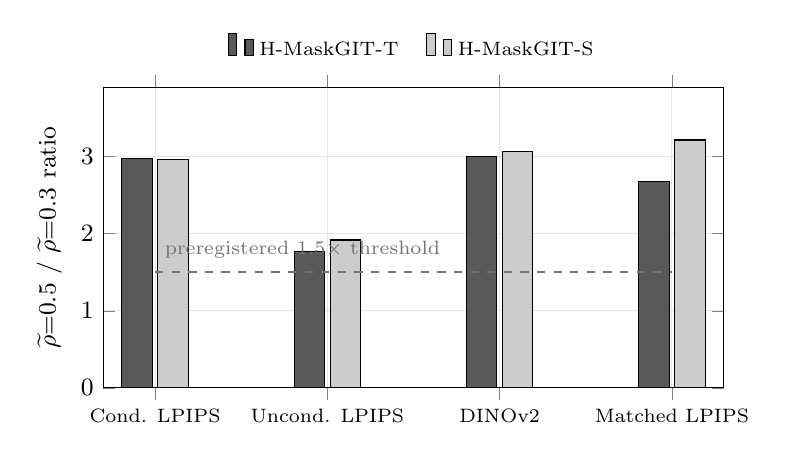
\begin{tikzpicture}
\begin{axis}[
  width=0.78\textwidth, height=5.4cm,
  ybar, bar width=11pt,
  symbolic x coords={Cond. LPIPS, Uncond. LPIPS, DINOv2, Matched LPIPS},
  xtick=data, ymin=0, ymax=3.9,
  ylabel={$\rholabel{=}0.5$ / $\rholabel{=}0.3$ ratio},
  legend style={at={(0.5,1.20)},anchor=north,font=\scriptsize,draw=none,
                legend columns=2,/tikz/every even column/.append style={column sep=8pt}},
  grid=major, grid style={gray!20},
  tick label style={font=\small}, label style={font=\small},
  x tick label style={font=\scriptsize}]
\addplot[fill=black!65,draw=black]
  coordinates {(Cond. LPIPS,2.975) (Uncond. LPIPS,1.775)
               (DINOv2,2.996) (Matched LPIPS,2.678)};
\addlegendentry{H-MaskGIT-T}
\addplot[fill=black!20,draw=black]
  coordinates {(Cond. LPIPS,2.963) (Uncond. LPIPS,1.919)
               (DINOv2,3.062) (Matched LPIPS,3.215)};
\addlegendentry{H-MaskGIT-S}
\draw[dashed,black!55,thick] (axis cs:Cond. LPIPS,1.5) -- (axis cs:Matched LPIPS,1.5);
\node[font=\scriptsize,anchor=south west,black!55] at (axis cs:Cond. LPIPS,1.55) {preregistered $1.5\times$ threshold};
\end{axis}
\end{tikzpicture}
\caption{Primary reverse-time ratios on two official checkpoints from the same
H-MaskGIT family. The dashed line marks the preregistered $1.5\times$ threshold.}
\label{fig:replication}
\end{figure}

% =====================================================================
\section{What the Data Do Not Support}
\label{sec:negative}

Several results constrain the claim, and reporting them is part of the claim.

\subsection{Measured influence profiles are only a coarse ordering}
Reachable-state q95 and calibration-maximum profiles achieve high finite-panel
coverage, but the clipped envelope they produce saturates in the early,
high-$\rholabel$ regimes where a bound would be most useful. Adding the static profile
to a structural baseline gives essentially no out-of-fold MAE improvement within
a fixed $\rho$. The profile works as a regime ordering and as a conservative
diagnostic, and it does not work as a certificate; Remark~\ref{rem:notcert}
anticipated the reason.

\subsection{W4 is saturated}
\label{sec:w4}
W4 direct TV is about an order of magnitude larger than W8, split incidence is
near one, and multi-seed events dominate. W4 confirms the direction of the
mechanism under a severe stress test, but the regime is far from the deployment
setting this paper is about, so we do not treat it as primary evidence.

\subsection{Source age is confounded}
Earlier-committed sources are associated with larger propagation under the frozen
selection rule. The association becomes unstable once source and shock
characteristics are adjusted for, so we make no causal claim about source age.

\subsection{No phase transition is established}
Damage increases sharply with the target anchor label $\rholabel$, but we neither fit nor test a discontinuous
changepoint. The correct term for what we measured is
\emph{reverse-time-dependent amplification}.

% =====================================================================
\section{Discussion}

\subsection{Why split frequency fails as a standalone risk metric}
A deployment monitor that reports only the probability of divergence will rank
the last decoding steps as the most dangerous, because those steps commit the
most positions at once. On our data that ranking is backwards for expected
consequence. The same approximate implementation has near-constant per-position
direct TV across reverse time, yet suffix sensitivity changes by more than an
order of magnitude. Expected damage is a product of onset and consequence, and
Section~\ref{sec:attribution} shows the two factors can carry opposite signs.

\subsection{What the instrumentation would enable next}
\label{sec:controller}
The experiments here use full suffix information, which makes them diagnostic
rather than a controller. What the instrumentation does provide is the separated
set of quantities a controller would need: the exact local split law, seed count
and severity, first descendant time, descendant growth, and final perceptual
consequence. A cost-saving system built on this should be held to a stricter
target than anything we test. Can \emph{pre-terminal} features identify the small
subset of transitions that deserve higher precision or recomputation? This paper
establishes the mechanism and the measurement contract and leaves that question
open.

\subsection{Where the theory and the experiments meet}
The stable-set theorem is the robust part. It holds at the architecture level and
needs only monotonicity and a branch-independent schedule. The
innovation--influence recursion shows how a finer bound could be built if global
local-sensitivity moduli were available, which for a neural decoder they are not.
The experiments then locate the useful interface: first-divergence onset and
conditional consequence carry the argument, while static influence profiles stay
secondary. That narrowing is itself a result. The closed-loop descendant count
turned out to be far more predictive than any static profile we measured.

% =====================================================================
\section{Limitations}

\begin{itemize}[leftmargin=1.4em,itemsep=3pt]
\item The two checkpoints belong to the same H-MaskGIT family, share the VQ
decoder, and use the same Halton scheduler. The results establish robustness
across checkpoint and scale, not generality across architecture families.
\item The joint law is defined by a specified coordinatewise conditional maximal
coupling. A different valid coupling can change paired path costs.
\item The natural-seed experiment is not persistent FP32-versus-W8 deployment.
After one FP32-versus-W8 transition, both branches use a common approximate
suffix (Section~\ref{sec:estimands}).
\item LPIPS, DINOv2, and the classifier diagnostics are operational metrics. No
human perceptual study is included.
\item The primary mechanism uses Halton with \texttt{randomize=False}. The
audited confidence sampler revises committed token values and would need a
different multitype theory.
\item We establish no global or tight neural influence certificate, no FID
improvement, no caching benefit, and no production safety guarantee.
\item The H-MaskGIT-S checkpoint bytes are external to the review archives.
Independent audit verifies the frozen ledger, revision, size, and SHA record, but
does not rehash the excluded 832\,MB file.
\end{itemize}

% =====================================================================
\section{Conclusion}

FDCA separates the onset of approximation-induced behavioral change from the
consequence that follows it. In masked visual generation the separation is not
cosmetic: W8 split incidence is highest late in decoding, while token and
perceptual damage conditional on a split is several times larger in earlier
states. Natural quantization seeds, common-suffix propagation, two paired
perceptual metrics, a matched same-shock control, and a second official
checkpoint all point the same way. For anyone monitoring an approximated
iterative generator, the practical consequence is that a divergence counter is
the wrong instrument on its own. Expected damage is the product of a split law, a
seed geometry, and the amount of generator state still to be decided.

% =====================================================================
\section*{Data, Code, and Version History}
\addcontentsline{toc}{section}{Data, Code, and Version History}

\paragraph{Release.} This document is version 1.0.0, the first public
archival release of the work. The venue-neutral layout and non-anonymous author
metadata are intentional for this technical-preprint record. Earlier numbered
manuscripts were internal development drafts and were not published as Zenodo
records, releases, or citable public versions.

\paragraph{Initial-public-release review.} Before this release, the manuscript
underwent a final correctness, scope, provenance, and artifact audit. The review
distinguished target anchor labels from attained unresolved fractions; stated
the batch-factorization and hybrid-closure assumptions; added zero-hazard and
zero-weight-row conventions; hardened Algorithm~\ref{alg:coupling} at
$\TV(p,q)=0$; recorded exact upstream and checkpoint configurations; completed
the H-MaskGIT-S prediction table; reconciled terminal-grid and package-manifest
arithmetic; incorporated directly relevant MaskGIT sampler work; and aligned the
paper, citation metadata, license, and public manifests. No frozen experimental
estimate or scientific gate was changed by this release-engineering pass.

\paragraph{Artifacts.} The initial public release contains the PDF, LaTeX and
BibTeX sources, machine-readable citation and Zenodo metadata, license, release
notes, and compact independent-audit reports. Large trajectory archives,
checkpoint weights, and metric weights are not redistributed here. The paper and
audit reports identify filenames, revisions, sizes, and SHA-256 ledgers.

% =====================================================================
% =====================================================================
\appendix
\section{Proofs}
\label{app:proofs}

\subsection{Proof of Theorem~\ref{thm:stableset}}
\begin{proof}
On $\{\tau = \dagger\}$ the two branches coincide at every step, so
$d(X_K,Y_K)=0$ and the bound holds trivially.

On $\{\tau \neq \dagger\}$ the two states are equal immediately before the first
split. Every coordinate in $F(X_{\tau-1})$ is equal at that time and is never
revised in either branch, so its terminal cost is zero. All terminal discrepancy
is therefore confined to the complement of $F(X_{\tau-1})$, and each surviving
coordinate cost is bounded by $\diam(c_u)$. Summing over $u \notin F(X_{\tau-1})$
gives the pathwise bound, and taking expectations gives the bound on $D^\Gamma$.
\end{proof}

\subsection{Proof of Proposition~\ref{prop:decomp}}
\begin{proof}
The events $\{\tau = k+1\}$ for $k = 0,\dots,K-1$ partition
$\{\tau \neq \dagger\}$, and $d_\lambda(X_K,Y_K)=0$ on $\{\tau=\dagger\}$. Hence
\[
  D^\Gamma = \sum_{k=0}^{K-1}
    \Ex\!\left[d_\lambda(X_K,Y_K)\,\Ind{\tau = k+1}\right].
\]
Condition on $G_k$ and on the common state $X_k=Y_k$. The conditional probability
of $\{\tau = k+1\}$ is $h_k(X_k)$ by definition, and the conditional terminal
cost on that event is $m_k(X_k)$. Applying the tower property term by term gives
the claim.
\end{proof}

\subsection{Proof of Theorem~\ref{thm:dag}}
\begin{proof}
Proceed in commit order and write $\pi_u = \Prob(X_K[u] \neq Y_K[u])$. When $u$
is committed, coordinatewise maximal coupling makes its mismatch probability
equal to $\TV\big(p_u(\cdot \mid X),\, q_u(\cdot \mid Y)\big)$. Insert the
intermediate law $q_u(\cdot \mid X)$ and apply the triangle inequality for total
variation. The same-state term is at most $s_u$ by definition. For the remaining
term, move from $X$ to $Y$ along a hybrid path that changes one previously
committed mismatched coordinate at a time; each single-coordinate change
contributes at most $M_{uv}$ and occurs with probability at most $\pi_v$, so the
accumulated state term is at most $\sum_{v \prec u} M_{uv}\pi_v$. Therefore
\[
  \pi_u \le \min\Big(1,\; s_u + \sum_{v \prec u} M_{uv}\pi_v\Big).
\]
The recursion defining $\bar r$ is monotone in its inputs, so induction over the
commit order gives $\pi_u \le \bar r_u$ for every $u$, and the weighted terminal
bound $D^\Gamma \le \lambda^\top \bar r$ follows by summation.

A position is influenced only by positions in strictly earlier commit blocks, so
$M$ is strictly block-triangular with $K$ blocks. Hence $M^K = 0$ and
$(I-M)^{-1} = \sum_{j=0}^{K-1}M^j$, which is where the unclipped version of the
envelope comes from. No contraction assumption is used anywhere.
\end{proof}

% ---------------------------------------------------------------------
\section{Experimental Program}
\label{app:program}

\begin{table}[h]
\centering
\caption{Stages that produced the final claim, in order.}
\label{tab:stages}
\small
\begin{tabular}{@{}>{\raggedright\arraybackslash}p{0.09\textwidth} >{\raggedright\arraybackslash}p{0.26\textwidth} >{\raggedright\arraybackslash}p{0.55\textwidth}@{}}
\toprule
Stage & Purpose & Outcome \\
\midrule
T0 & Exact finite-state theorem and code validation &
Stable-set bound, clipped envelope, Wasserstein ordering, and the
fresh-innovation counterexample all pass. \\
P0 & Official sampler contract &
Halton is branch-independent and token-value monotone; the confidence sampler is
monotone in occupancy only. \\
P05R & Real-model influence microaudit &
Profiles tighten the late regimes but fail uniform global criteria; the profile
is demoted to a secondary diagnostic. \\
P1L & Controlled single shock &
Strong reverse-time token amplification and spatial spread. \\
P1M & Model-free incremental analysis &
Profile adds little within-anchor value; the regime-level result is robust. \\
P2N & Natural W8 seed bridge &
Exact incidence, natural seed, conditional propagation, and matched timing all
supported. \\
P2A/P2B & RNG, MASK, and clamp closure &
Unclassified key duplicates 0; hidden MASK and clamp artifacts excluded. \\
P2P & Perceptual bridge &
LPIPS, DINOv2, token link, and matched timing (H1--H5) all pass. \\
P3S & Second checkpoint &
R1--R4 and the token link replicate on H-MaskGIT-S. \\
\bottomrule
\end{tabular}
\end{table}

The T0 counterexample referenced in Section~\ref{sec:estimands} is a finite-state
chain on which a seed-only recursion, applied to the persistent-approximation
estimand, strictly underestimates the terminal cost. It is the reason the two
estimands are kept apart throughout the paper.

% ---------------------------------------------------------------------
\section{Full H-MaskGIT-T Perceptual Tables}
\label{app:tables}

Table~\ref{tab:fullT} gives the conditional and exact incidence-weighted
outcomes at every anchor. Conditional columns answer "how bad if it splits";
unconditional columns are the conditional value multiplied by the exact incidence
of the same row, following Proposition~\ref{prop:decomp}. Reading across a row
shows the two directions cancelling; reading down the unconditional LPIPS column
shows that the cancellation is incomplete.

\begin{table}[h]
\centering
\caption{Conditional and exact incidence-weighted perceptual outcomes by
reverse-time anchor (H-MaskGIT-T, W8, 48 blocks).}
\label{tab:fullT}
\scriptsize
\setlength{\tabcolsep}{3pt}
\begin{tabular}{@{}cccccccc@{}}
\toprule
$\rholabel$ & $\rhoatt$ & Split incidence & Cond.\ LPIPS & Uncond.\ LPIPS
& Cond.\ DINOv2 & Uncond.\ DINOv2 & Cond.\ JSD \\
\midrule
0.1 & 0.1602 & 0.50079 & 0.004441 & 0.002267 & 0.003435 & 0.001699 & 0.000611 \\
0.3 & 0.2813 & 0.21323 & 0.010126 & 0.002213 & 0.007432 & 0.001512 & 0.001558 \\
0.5 & 0.4922 & 0.12976 & 0.030126 & 0.003927 & 0.022270 & 0.002830 & 0.004861 \\
0.7 & 0.6914 & 0.10207 & 0.075937 & 0.007869 & 0.056340 & 0.005639 & 0.010492 \\
0.9 & 0.9023 & 0.08329 & 0.214513 & 0.017798 & 0.152405 & 0.012133 & 0.024952 \\
\bottomrule
\end{tabular}
\end{table}

\begin{table}[h]
\centering
\caption{Seed geometry and propagation at the two preregistered anchors
(H-MaskGIT-T, W8).}
\label{tab:seedgeom}
\small
\begin{tabular}{@{}lcc@{}}
\toprule
Quantity & $\rholabel=0.3$ & $\rholabel=0.5$ \\
\midrule
Positions in next commit batch & 14 & 8 \\
Exact split incidence & 0.2132 & 0.1298 \\
Expected seed count $\Ex|S_{\mathrm{seed}}|$ & 0.2382 & 0.1379 \\
Share of splits with exactly one seed coordinate & $\approx 89\%$ & $\approx 94\%$ \\
Conditional descendant rate & 0.0375 & 0.0848 \\
\bottomrule
\end{tabular}
\end{table}

\begin{table}[h]
\centering
\caption{Leave-one-block-out prediction of terminal LPIPS. The seed-only model
uses the target-anchor category, seed count, direct-TV severity, surprisal, and seed topology; the
propagation model adds descendant count and rate, first descendant step, and
spatial spread. The replication entries come from the frozen P3S out-of-fold audit.}
\label{tab:lobo}
\small
\begin{tabular}{@{}lcc@{}}
\toprule
Quantity & H-MaskGIT-T & H-MaskGIT-S \\
\midrule
Seed-only held-out MAE & 0.03035 & 0.01280 \\
Propagation held-out MAE & 0.01568 & 0.006964 \\
MAE ratio & 0.5166 & 0.5440 \\
Bootstrap interval for the MAE improvement & $[0.01240,\ 0.01702]$ & $[0.004914,\ 0.006790]$ \\
Within-regime residual Spearman & 0.368 $[0.313,\ 0.423]$ & 0.584 $[0.501,\ 0.664]$ \\
\bottomrule
\end{tabular}
\end{table}

% ---------------------------------------------------------------------
\section{Reproducibility and Audit Notes}
\label{app:audit}

\paragraph{Block independence.} Every scientific stage uses deterministic
class--seed manifests and excludes all predecessor blocks. The primary perceptual
study uses 48 new blocks; the replication uses 40 new blocks chosen by a
preregistered power calculation.

\paragraph{Zero controls.} Zero-seed controls produce identical pre-clamp and
post-clamp token grids, identical decoded image hashes, and exactly zero LPIPS,
DINOv2, and classifier distance. These controls exercise the whole
coupling--decode--metric pipeline rather than the token sampler alone, which is
why they are run at the same scale as the scientific panels.

\paragraph{MASK and clamp.} A targeted replay retains every equal and mismatched
token pair at the natural seed transition. Across more than two million selected
token pairs, no equal-MASK and no one-sided-MASK event occurs. The perceptual
panels record zero selected-MASK events and zero clamp-induced changes.

\paragraph{RNG.} The semantic key registry classifies intentional cross-cell
reuse of the reference proposal stream and fails on any unclassified duplicate.
The final primary and replication panels contain zero unclassified, missing, or
unexpected keys.

\paragraph{Artifact integrity.} Run manifests are non-self-referential and carry
size and SHA entries. The P2P independent analysis clean-extracts the Full
package and reproduces the gate. Its 2,496 terminal grids decompose as 1,920 W8
natural pairs, 192 W4 stress pairs, 96 matched-timing pairs, and 288 zero
controls. The P3S 1,040 grids decompose as 640 primary natural pairs, 160 matched
timing pairs, 80 primary zero controls, 128 official-CFG sensitivity pairs, and
32 sensitivity zero controls. The P3S independent audit verifies the Full,
Summary, and run manifests, all headline arithmetic, the zero controls, the
logging rows, the source code, and a secondary implementation. Its Full package
contains the 1,429 run-manifest files plus two archive-level bookkeeping files.

% ---------------------------------------------------------------------
\section{Claim--Evidence Matrix}
\label{app:claims}

\begin{table}[h]
\centering
\small
\caption{Every claim in the paper with its evidential status.}
\label{tab:claims}
\begin{tabular}{@{}p{0.32\textwidth} p{0.14\textwidth} p{0.45\textwidth}@{}}
\toprule
Claim & Status & Evidence and qualification \\
\midrule
Stable-set first-divergence bound & Theorem & Fixed monotone common schedule. \\
Coordinate clipped envelope & Theorem & Requires global admissible-state
innovation and influence moduli. \\
Measured influence profile is tight & Not supported & Conservative, saturates
early, weak within-anchor prediction. \\
Natural W8 seed propagates & Supported & P2N; common W8 suffix, specified
coupling. \\
Reverse-time token amplification & Supported & Controlled shock, natural seed,
matched timing. \\
Perceptual reverse-time amplification & Supported & LPIPS and DINOv2 on
H-MaskGIT-T and H-MaskGIT-S. \\
Token propagation predicts LPIPS & Supported & Leave-one-block-out improvement on
both checkpoints; not an online early-warning model. \\
Source age causes propagation & Not supported & Association is confounded and
unstable under adjustment. \\
Human perceptual failure & Untested & Operational metrics only. \\
Persistent deployment guarantee & Untested & One-step natural seed plus common
suffix. \\
Architecture-family generality & Untested & Two checkpoints in one H-MaskGIT
family. \\
Coupling-universal result & Untested & Coordinatewise conditional maximal
coupling. \\
\bottomrule
\end{tabular}
\end{table}

% ---------------------------------------------------------------------
\section{Terminology Checklist}
\label{app:terms}

The following distinctions are load-bearing and are applied consistently above.

\begin{itemize}[leftmargin=1.4em,itemsep=2pt]
\item Write \emph{reverse-time-dependent amplification}, not \emph{phase
transition}.
\item Write \emph{operational perceptual distance}, not \emph{human perceptual
failure}.
\item Name the specified coupling whenever a paired damage number is reported.
\item Keep \emph{exact split incidence under the specified coordinatewise
coupling}, \emph{split-conditional consequence}, and
\emph{incidence-weighted consequence} separate
(Section~\ref{sec:threenumbers}).
\item Keep the \emph{natural one-step seed plus common suffix} estimand separate
from \emph{persistent approximation} (Section~\ref{sec:estimands}).
\item Report measured influence profiles as finite-panel diagnostics, never as
global certificates (Remark~\ref{rem:notcert}).
\item Keep W8 as the primary realistic regime and W4 as a saturated stress panel.
\item Distinguish target anchor label $\rholabel$ from attained unresolved
fraction $\rhoatt$.
\end{itemize}

% =====================================================================
\bibliography{references}

\end{document}
